\unnumberedChapter{Base Station Hardware}

The base station is essentially based on a main controller board, a power module unit and a RailCom detector. We will use the PICO controller building block shown in the previous chapter. The extension connector of the base station exports the I2C interface and the DCC signal produced by the base station. So, adding an I2C based extension board for display, switches, etc. is possible. The following figure depicts the overall block diagram.

\begin{figure}[htbp]
    \centering
    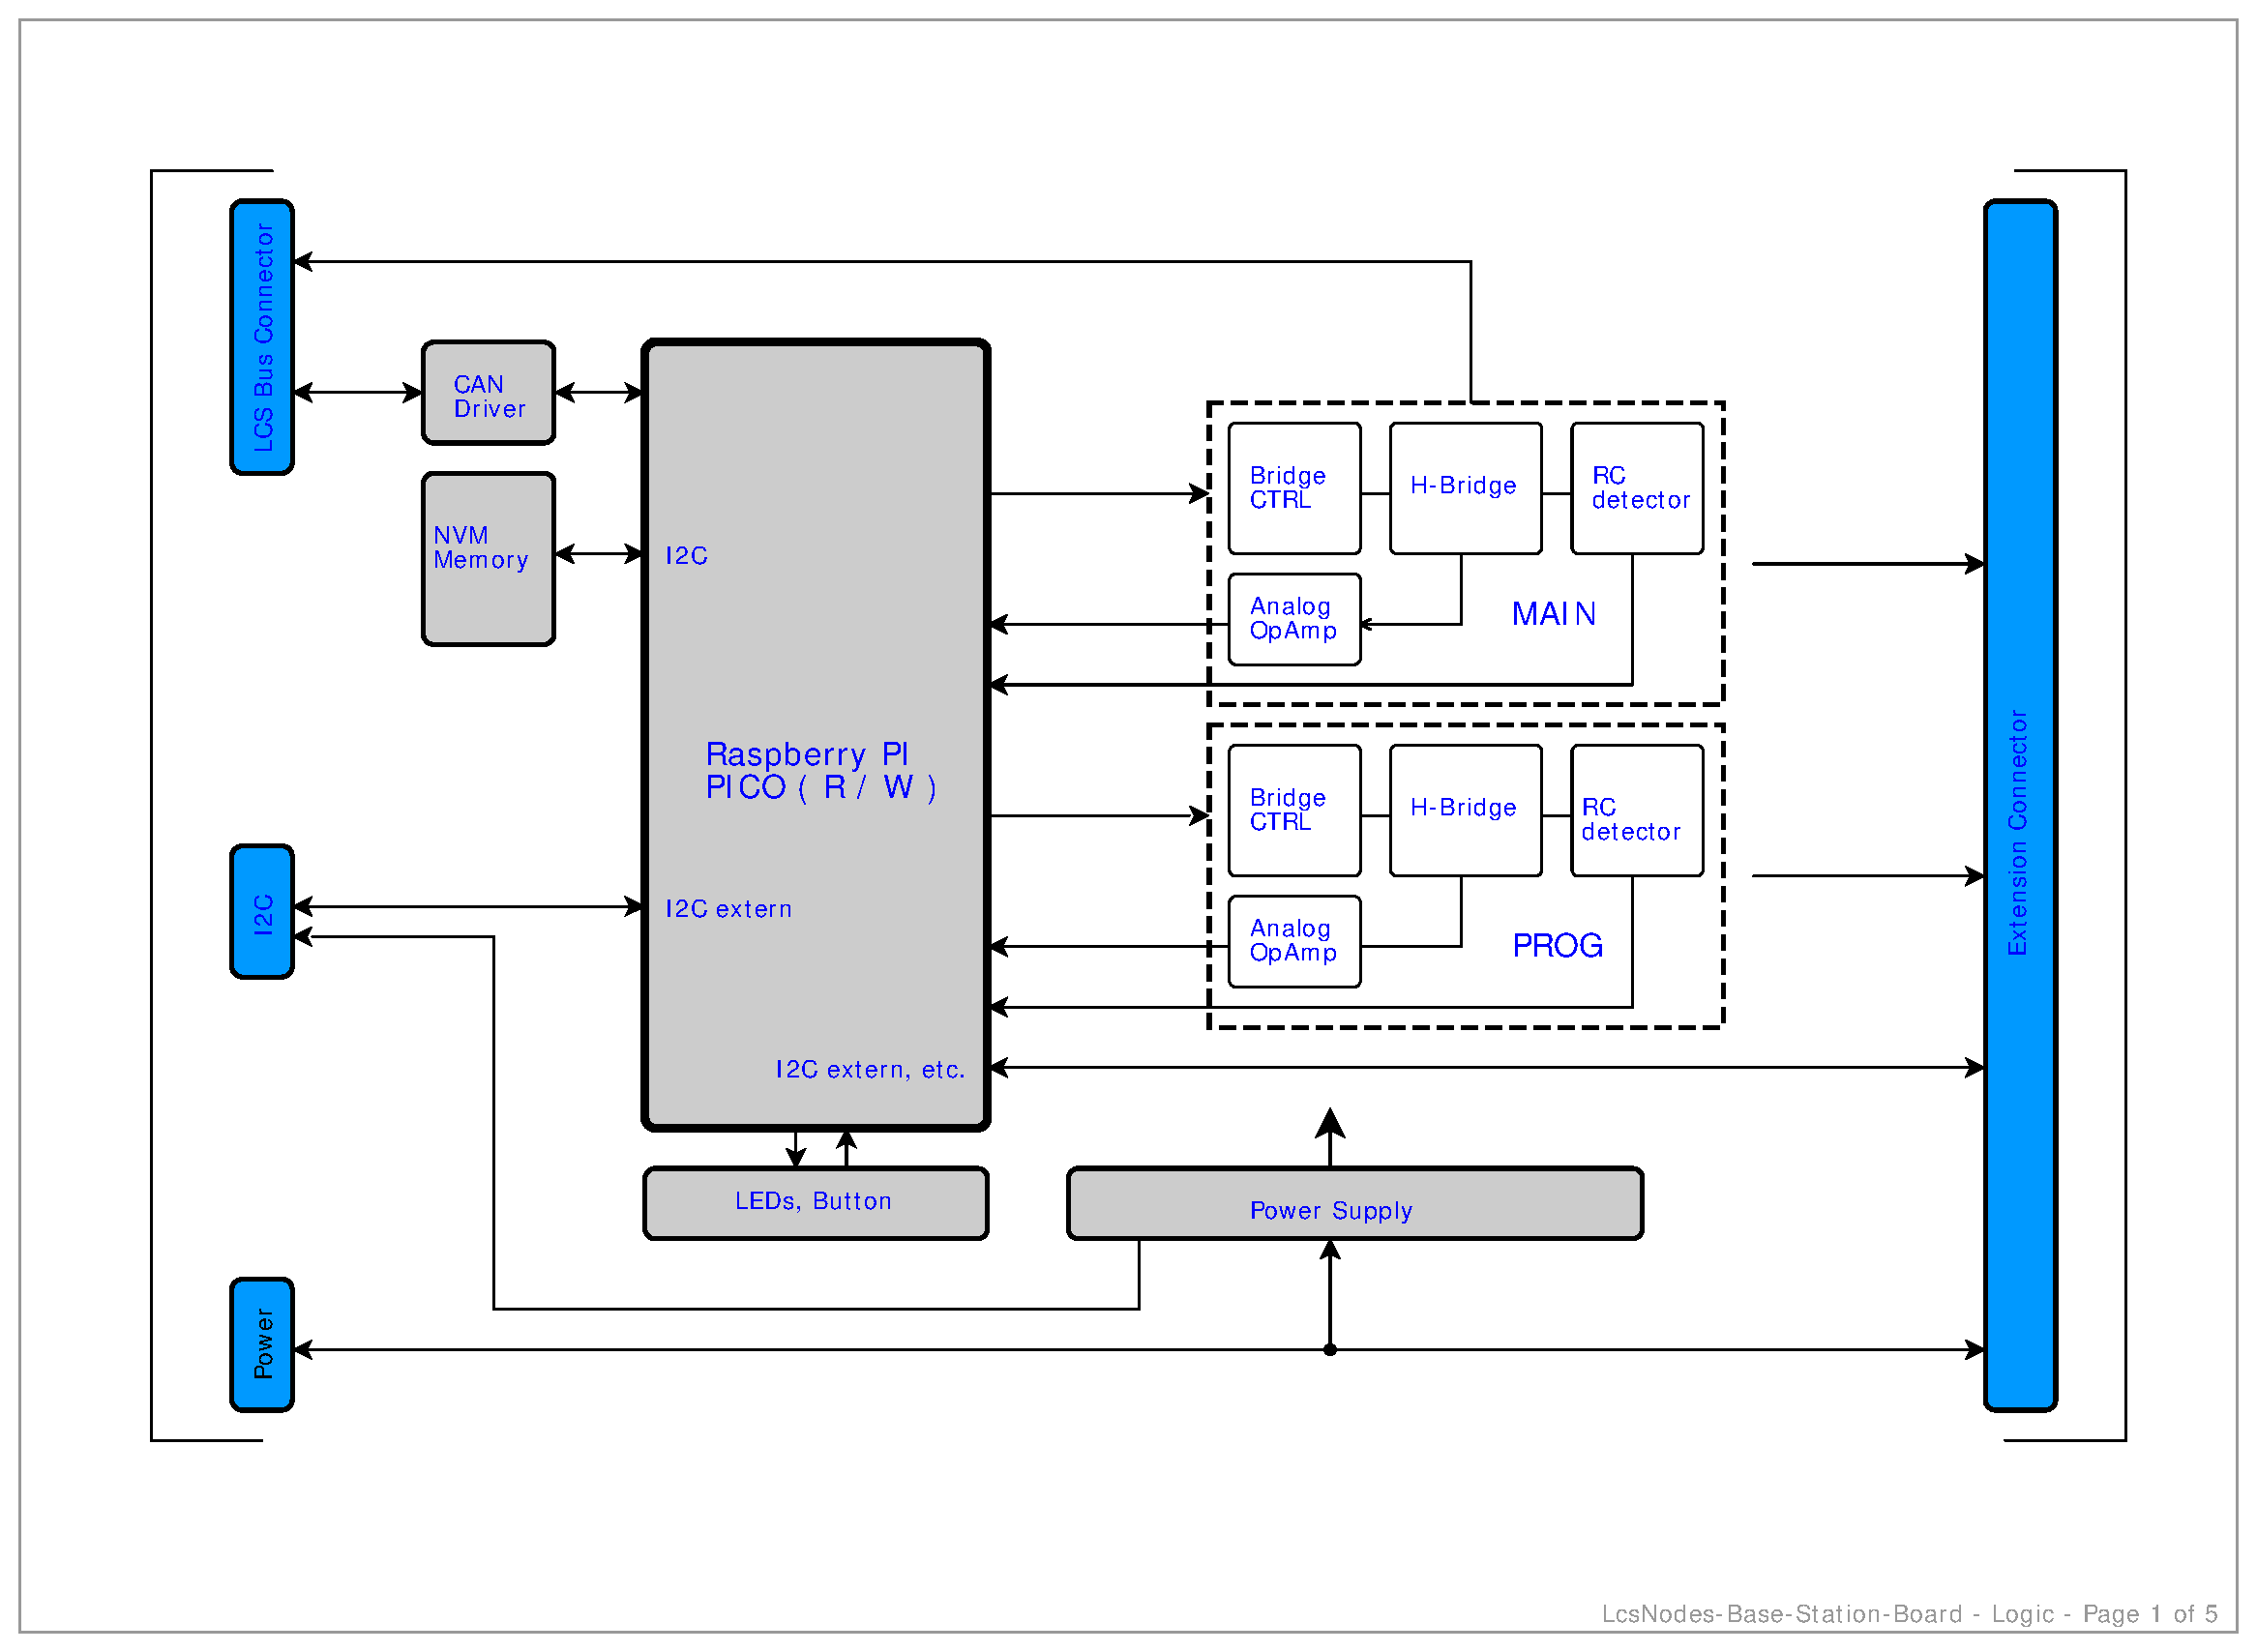
\includegraphics[page=1, width=0.9\textwidth]{./part-base-station/chapter-base-station-hardware/Schematic_LcsNodes-Base-Station-Board-B.02.10.pdf}
    \caption{Base Station Block Diagram}
    %\label{fig:BlockDiagram}
\end{figure}
\FloatBarrier

As said, there are two more building blocks we have to introduce first. They are the \texttt{power unit} and the \texttt{RailCom detector}.

\unnumberedSection{Power Module}

A layout control system needs a form of DCC signal generator. They can be directly integrated with the base station to form one hardware module or be at the heart of a separated booster module. Depending on the model railroad scale, there are different voltages and maximum current considerations. A Gauge N layout has a different power requirement than a Gauge G layout. The NMRA standard defines the voltage ranges for the different gauges. Our assumption is that the layout system has a form of power supply that delivers the voltage and current requirements to the power module. For convenience, all hardware module node local power supplies for the controller and other chips should be able to handle a voltage range between 7V and 24V when drawing power from this power supply.

The power module exports the DCC signals via the external connectors and also as part of the LCS message bus connector. The track power extension connector is used by extension boards that directly use the H-Bridge output. A good example is an occupancy detector board which takes the DCC outputs and routes them to different sections, each equipped with a detectors for power consumption on the track. The power module unit features two identical channels. They are labelled "MAIN" and "PROG". Although the "PROG" channel would not need to deliver a high amperage, the dual H-Bridge is there anyway. And as said before, it would be nice to dynamically treat the PROG track as a type MAIN track too. 

 The main task of the DCC track power module is to provide the DCC signal to the track. DCC signals are square wave signals with a defined duty cycle period. A duty cycle of 58 microseconds represents a "DCC one", a duty cycle of 116 microseconds a "DCC zero" bit. A typical solution to this task is a H-Bridge design. The following figure shows the H-Bridge signal convention for LCS power modules.
 
 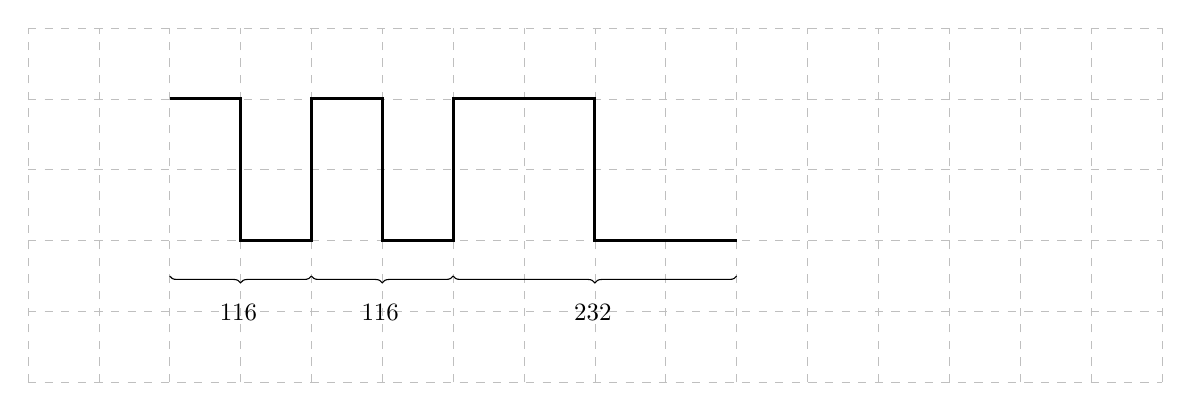
\begin{tikzpicture}[scale=0.9, transform shape]

    \draw[help lines, gray!50, dashed] (0,-2) grid (16,3);

    % Square wave

    \draw[line width=1pt]

        (2,2) -- (3,2) -- (3,0) -- (4,0) -- (4,2)
        -- (5,2) -- (5,0) -- (6,0) -- (6,2)
        -- (8,2) -- (8,0) -- (10,0);

    % Braces

    \draw[decorate, decoration={brace, mirror}]

        (2,-0.5) -- (4,-0.5)
        node[midway, below=8pt] {116\,\si{\micro\second}};

    \draw[decorate, decoration={brace, mirror}]

        (4,-0.5) -- (6,-0.5)
        node[midway, below=8pt] {116\,\si{\micro\second}};

    \draw[decorate, decoration={brace, mirror}]

        (6,-0.5) -- (10,-0.5)
        node[midway, below=8pt] {232\,\si{\micro\second}};

\end{tikzpicture}


While a power module can vary in capacity and technology components, our logical design expect to send the same digital signals to a power module, no matter what it's design. It is a key requirements to derive from the DCC signal on the bus connector the state "+", "-" and "short circuit". The latter is needed for the cutout option. There is also the need to detect a logic "one" on both signal inputs and interpret this as setting the bridge to a high impedance state. This requirement comes primarily from the capability to also issue PWM signals, which will depending in the direction alternate between a positive or negative voltage and the high impedance state. There is a whole family of H-Bridge ICs and breakout boards. If a particular H-Bridge IC does not map the inputs to the table below, some gate logic needs to be added. The following table depicts the power module digital input management signals. The table below fits the L6205 H-Bridge nicely.

\begin{longtable}{@{}|l|l|l|p{0.4\linewidth}|@{}}
    %\caption{Bus Connector Pins}
    \toprule
    \textbf{Enable} & \textbf{DCC-Sig-1} & \textbf{DCC-Sig-2} & \textbf{Meaning} \\
    \midrule
    \endfirsthead
    \toprule
    \textbf{Enable} & \textbf{DCC-Sig-1} & \textbf{DCC-Sig-2} & \textbf{Meaning} \\
    \midrule
    \endhead
    \midrule
    \multicolumn{2}{r}{\textit{Continued on next page}} \\
    \midrule
    \endfoot
    \bottomrule
    \endlastfoot
    1 & 0 & 0 & Cutout period. The track will be short circuited. OUT1 and OUT2 are connected to ground. \\
    \midrule
    1 & 1 & 0 & The track is polarized "+". OUT1 is connected to VS, OUT2 is connected to GND. \\
    \midrule
    1 & 0 & 1 & The track is polarized "-". OUT1 is connected to GND, OUT2 is connected to VS. \\
    \midrule
    X & 1 & 1 & The track is put into high impedance, i.e. not connected. \\
    \midrule
    0 & X & X & The track is put into high impedance, i.e. not connected. \\
\end{longtable}

The standards also specify which side of the track is the positive side, i.e. OUT1 in the table above. The right hand track side, usually connected with a red cable is the positive side, the left track side, connected with a black cabe, is the negative side. If the H-Bridge is enabled, sending a "DCC One" will mean to raise the digital output of the controller port DCC-SIG-1 to HIGH and controller port DCC-SIG-2 to LOW for 58 microseconds, followed by the reverse bit setting for another 58 microseconds. The DCC packet is broken down, bit by bit and the digital signal is produced. The H-Bridge hardware then takes the zero and ones and essentially reverses the track polarity accordingly to digital zeroes and ones.

If the power bridge is used for the PWM mode, a "FWD" means to raise  the DCC-SIG-1 to HIGH and the controller port DCC-SIG-2 to LOW for the active part of the duty cycle length. The remainder of the duty cycle, the port signals will be both set to a HIGH, which puts the bridge into the high impedance state. Not all H-Bridge ICs follow the same control signal level standard. Any difference in H-Bridge control signals inout logic need to be masked accordingly. The following figure shows the H-Bridge signal standard. All power modules and connectors to the track follow this convention.

All power modules are expected to deliver a voltage proportional to the power consumption of the H-Bridge. This is typically done by putting a shunt resistor between ground and the lower part of the H-bridge. For a better accuracy, the rather low voltage signal is amplified before delivered to the analog input of a controller. Note that most H-Bridge ICs offer short circuit and over temperature protection already as a built-in feature. Based on the analog voltage signal analysis, current protection features such as sending a power overload event can be implemented.

Power consumption measurement is necessary for another important DCC requirement. A DCC decoder in programming mode will raise its power consumption to acknowledge an operation with a raise by about 60mA. This short rise needs to be detected as well. It requires to calibrate the actual power consumption of the decoder, build a base of typical consumption and then detect the temporary raise. With the basics in place now, the next section will show different designs for a power module using the L6205 chip for the implementation. As always, there are other H-Bridges and also breakout boards that could also be used as the heart of a power module building block.

Finally, there is support for short circuit detection and protection. The L6205 H-Bridge stops in microseconds on a shirt circuit detection. We can hardly detect that by power consumption measurement and will see a zero consumption on our periodic measurement. So, as long we measure within in the defined power limit and stay below a real short circuit, we are fine. On a short circuit, the chip does a much better job. Fortunately the L6205 chip sends a signal for a short circuit. We feed this direct to a controller pin for short circuit processing.


\unnumberedSection{DCC and RailCom Signal Detector}

Although a possibly standalone component in a layout, the RailCom detector is typically also a part of the base station. It sits between the power module and the track. DCC is a broadcasting protocol. To address programming engines on the MAIN track the problem of providing a back channel had to be solved. First, the DCC signal generator needs to be able to include a cutout period in the bitstream. 

As shown in the DCC subsystem chapter, the cutout period happens right after the last bit of a packet sent as part of the preamble section of the next packet. The power module short circuits the track during this period. The decoder uses the period to send a short bit stream which in turn is detected by the RailCom detector. This section will just discuss the hardware part for receiving the RailCom bitstream in the cutout period. There is of course a software part that receives and decodes the RailCom datagrams. The details of RailCom message processing are described in the base station chapter.

\begin{tikzpicture}[scale=0.9, transform shape]

    \draw[help lines, gray!50, dashed] (0,0) grid( 16,4);
    \node at (8,4) {picture};

\end{tikzpicture}

The RailCom channel was an important addition to the DCC standard. With RailCom capable decoders data can be queried and set while the engine is on the main track. This chapter showed a simple building block that allows to detect a RailCom stream. It is actually a very modest hardware addition, so that each H-Bridge delivering DCC signals should be equipped with such a detector. We will make use of this building block for all power modules found in the base station and block controller designs.


\unnumberedSection{Base Station Main Controller}

The schematic parts of the base station main controller should be familiar. Exactly, they are almost an exact copy of the genric main controller... 


\begin{figure}[htbp]
    \centering
    \includegraphics[page=2, width=0.9\textwidth]{./part-base-station/chapter-base-station-hardware/Schematic_LcsNodes-Base-Station-Board-B.02.10.pdf}
    \caption{Base Station Main Controller}
    %\label{fig:Schematic}
\end{figure}
\FloatBarrier


\unnumberedSection{Power Unit}

The power unit of our base station uses the L6205 dual H-Bride IC for a dual power module unit. There is a serial resistor on bridge ground side to measure the current consumption. The voltage drop over this resistor is amplified and will be passed to an analog controller pin. Both bridges deliver up to 2.8A, which is sufficient for scales up to HO or O and 1 Gauge Scale for smaller locos.


\begin{figure}[htbp]
    \centering
    \includegraphics[page=3, width=0.9\textwidth]{./part-base-station/chapter-base-station-hardware/Schematic_LcsNodes-Base-Station-Board-B.02.10.pdf}
    \caption{Power Module}
    %\label{fig:Schematic}
\end{figure}
\FloatBarrier

When building a base station, one H-bridge is used or the main track and the other for the programming track. The programming track actually would need a much lower current, so why use a design with two equally powered H-bridges? One answer is that you can get such an ICs with two H-Bridges inside. The other answer is that a design with two equal H-Bridges would allow for an interesting feature. Imagine you could feed the main track signal to both the MAIN and the PROG track. A locomotive could drive under its own power onto the PROG track, which is acting as a MAIN track section. Then the DCC signal is switched back from MAIN to PROG and the locomotive configuration can begin. Now, the same could also be accomplished with some relay based logic, but wouldn't this be an elegant approach? The hardware is there.


\unnumberedSection{RailCom Detector}

Both channels also feature a RailCom detector. 


\begin{figure}[htbp]
    \centering
    \includegraphics[page=4, width=0.8\textwidth]{./part-base-station/chapter-base-station-hardware/Schematic_LcsNodes-Base-Station-Board-B.02.10.pdf}
    \caption{RailCom Detector}
    %\label{fig:Schematic}
\end{figure}
\FloatBarrier


// ??? what else to say here...

Refer to the base station firmware chapter on what we actually do with a RailCom detector. 


\unnumberedSection{ Connectors and Power}

Finally, there are the connectors and the power supplies. There are the standard LCS Can bus connectors and the external I2C channel connector. On the left side, there is the 60-pin connector for possible extension boars. 

\begin{figure}[htbp]
    \centering
    \includegraphics[page=5, width=0.8\textwidth]{./part-base-station/chapter-base-station-hardware/Schematic_LcsNodes-Base-Station-Board-B.02.10.pdf}
    \caption{Connectors and Power}
    %\label{fig:schematic}
\end{figure}
\FloatBarrier

// ?? external connector offers just a few lines out ...

The power supply ....


\unnumberedSection{Base Station PCB}

The following picture shows the PCB for the LCS base station. It is a 12cm by 10cm board, with the standard connectors in the usual place. 



\begin{figure}[htbp]
    \centering
    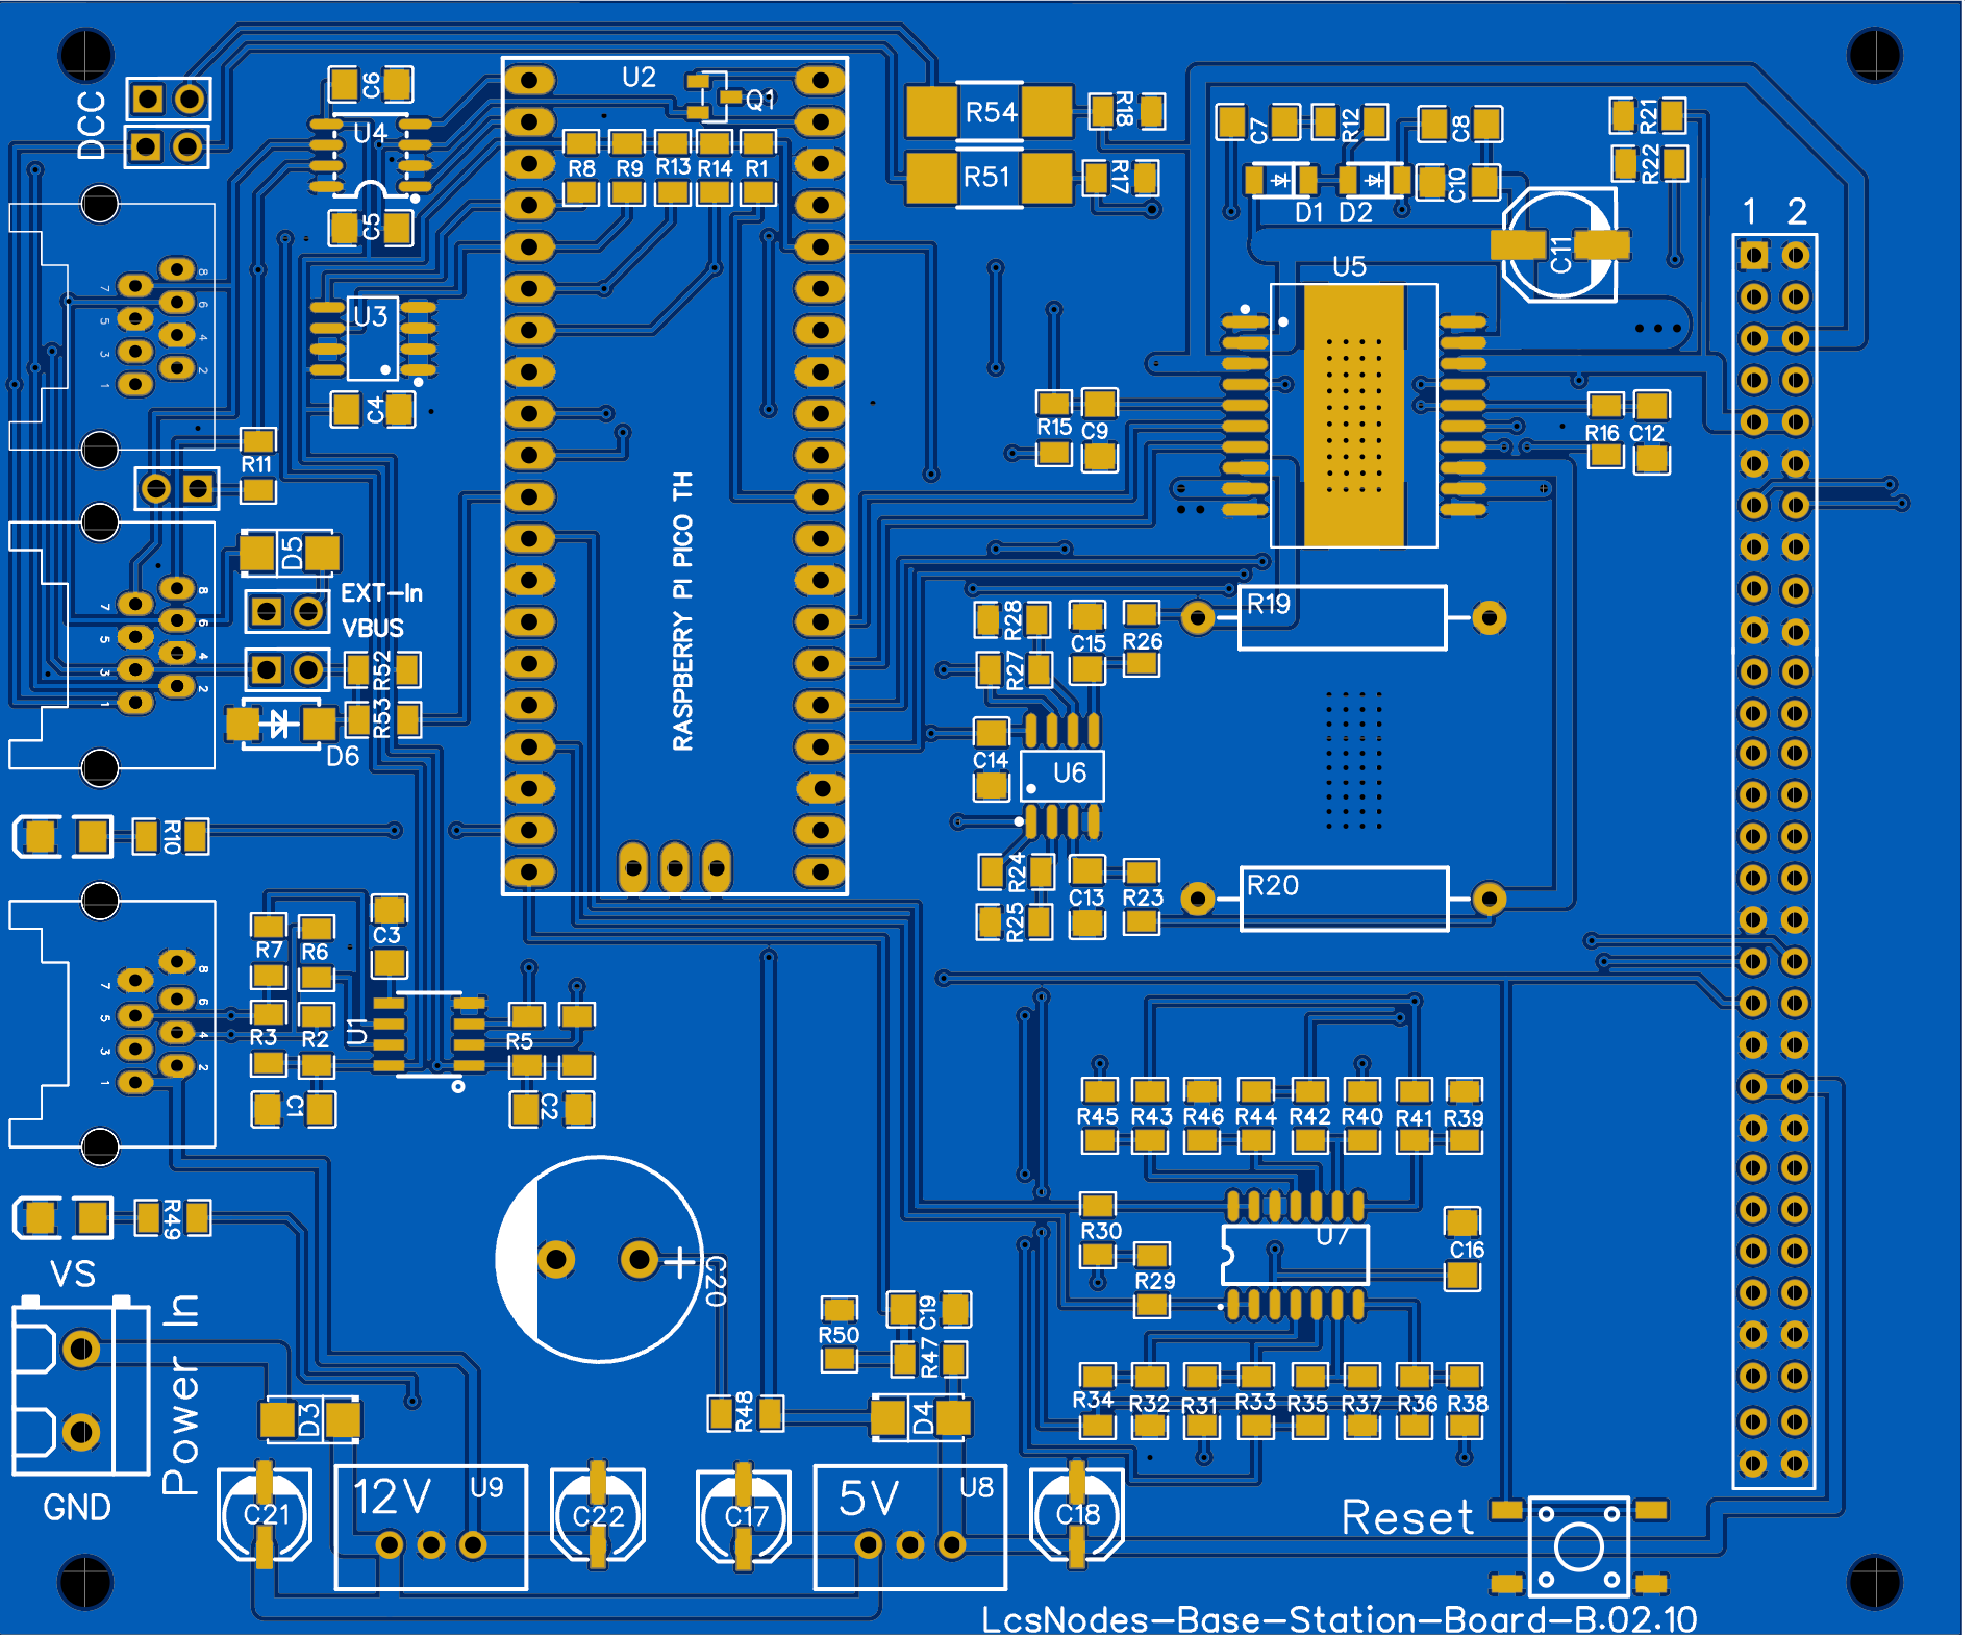
\includegraphics[width=0.8\textwidth]{./part-base-station/chapter-base-station-hardware/PCB_LcsNodes-Base-Station-Board-B.02.10.pdf}
    \caption{Base Station}
    %\label{fig:schematic}
\end{figure}
\FloatBarrier

\unnumberedSection{A little history}

The base station was also the first major LCS node with a considerable amount of hardware and software and thus went to several iterations and a fair amount of learning curves. The very first version started with an Arduino Mega and Motor driver breakout board. The software was the original DCC++ software. The next versions actually were just refactoring efforts and work on the software. I learned a great deal on how all this works. The next base station version was a single board with all possible interfaces on an experimental PCB. It already featured CAN BUS, dual H-Bridges, and a controller, the Atmega 1284. This board served a long time for software development and further experiments. 

The next version of the base station was built with a main controller PCB described in the earlier chapters and a dual power unit, that also featured the RailCom detector. And again further software refactoring, refinement and learning. Finally, after a switch to the Raspberry Pi Pico controller, first on breadboard  then on PCBs, the base station shown in this chapter is the current version. The lessons learned proved to be very valuable for the overall concept development and hardware design. And in addition, there was a great deal of reading on chip specifications and, very importantly, the DCC standards. The appendix contains a list of material and web links. I highly recommend to read the electrical and DCC related standards published by the RailCommunity organization.

Another significant effort was the switch from the Arduino IDE and universe to vsCode with cMake. The entire project setup is in one GIT repository and changing a byte in any library results in a consistent re-build of all components. 


\unnumberedSection{Summary}

The base station, no matter how it is implemented, is a key component in any digital layout. It is primarily responsible for the locomotive session management and track signal generation. There could be designs where the base station is a device in a nice housing with a display, switches and so on. Other designs just put the LCS node somewhere on the layout. All these options will work just fine. And just like any other LCS node, the base station firmware offers through node and port attributes status and control functions. The base station firmware is next.



